\documentclass{beamer}
\mode<presentation>{\usetheme{Warsaw}}
\usepackage[english]{babel}
\usepackage[utf8x]{inputenc}
\usepackage[T1]{fontenc}
\usepackage{hyperref}

\title{Advanced Algorithms and Parallel Programming Spring 2018}
\subtitle{Advanced Algorithms Project}
\author{Semsi Yigit Ozgumus}
\institute{Politecnico di Milano}
\date{\today}

\AtBeginSection[]
{
	\begin{frame}
	\frametitle{Current Section}
	\tableofcontents[currentsection]
	\end{frame}
}

\setbeamertemplate{sidebar right}{}
\setbeamertemplate{footline}{%
\hfill\usebeamertemplate***{navigation symbols}
\hspace{1cm}\insertframenumber{}/\inserttotalframenumber}

\begin{document}
	\begin{frame}
		\titlepage
	\end{frame}

	\begin{frame}
		\frametitle{Table of Contents}
		\tableofcontents
	\end{frame}
	
	\section{Introduction of the Problem}
		\begin{frame}
			\frametitle{What is a Strongly Connected Component ?}
			
			\begin{itemize}
				\item<2-> if a Vertex is reachable by any vertex in the graph, then that vertex is \textbf{strongly connected}.
				\item <3-> if a partition of vertices that are a subgraph of the graph are all strongly connected, then that subgraph is a \textbf{strongly connected component} of that graph.
				\item <4-> 	\begin{figure}[h!]
					\centering
					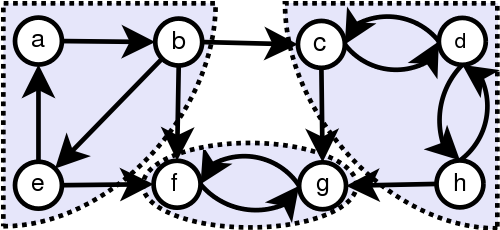
\includegraphics[width=.6\textwidth]{scc}
					\caption{Graph with strongly connected components}
				\end{figure}
			\end{itemize}
		\end{frame}
		
		\begin{frame}
			\frametitle{Methods to solve}
			\begin{itemize}
				\item <2-> Tarjan's Algorithm
				 \begin{itemize}
					\item <3-> Time Complexity $\rightarrow O(| V | + | E |)$
					\item <4-> Space Complexity $\rightarrow O(|V| \cdot (2 + 5 w)) $
				\end{itemize}
				\item <5-> Nuutila's Version
					\begin{itemize}
						\item <6-> Space Complexity  $\rightarrow O(|V| \cdot (1 + 4 w)) $
					\end{itemize}
				\item <7-> Pearce's Version
					\begin{itemize}
						\item <8-> Space Complexity  $\rightarrow O(|V| \cdot (1 + 3 w)) $
					\end{itemize}
			\end{itemize}
		\end{frame}
	
	\section{Implementation of the Project}
		\begin{frame}
			\frametitle{Project Structure}
			\begin{itemize}
				\item <1-> In terms of functionality the project has 4 different functions.
				\begin{enumerate}
					\item <2-> Generate a Random Directed Graph with options (Python)
					\item <3-> Run Experiement with algoritmhs while keeping track of completion time and storage consumption (tarjan vs. Nuutila vs. Pearce)(C++)
					\item <4-> Debug mode for testing a singular graph with algorithms provided(C++).
					\item <5-> Visualization of the experiments, can only be done with cvs files (Python).
				\end{enumerate}
			\end{itemize}
		\end{frame}
		\begin{frame}
			\frametitle{Project Structure}
			\begin{itemize}
				\item <1-> All the steps are connected to each other and glued together to create a pipeline to emulate terminal application.
				\item <2-> All documentation done in Doxygen
				\item <3-> Visualization of the experiment is done with python, csv files can be further explored using the provided jupyter notebook.
			\end{itemize}
		\end{frame}
		\subsection{Python}
		\begin{frame}
			\frametitle{Python Part}
			\begin{itemize}
				\item <1-> There are 2 scripts that are embedded into the project.
				\begin{enumerate}
					\item <1-> generate\_graph\_directories.py
					\item <2-> analysis.py
				\end{enumerate} 
				\item <3-> They can be used outside of application
			\end{itemize}
		\end{frame}
		\begin{frame}
			\frametitle{Python Part}
			\begin{figure}[h!]
				\centering
				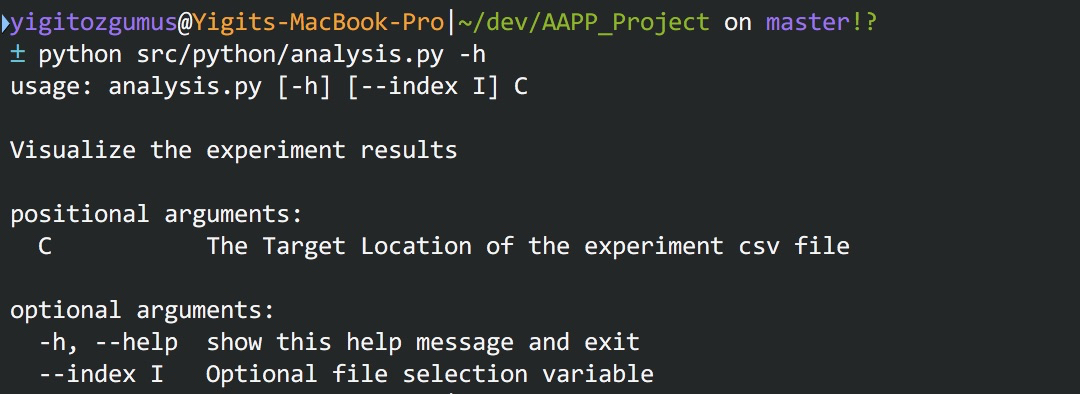
\includegraphics[width=1\textwidth]{analysis}
				\caption{Analysis script help command result}
			\end{figure}		
		\end{frame}
		\begin{frame}
			\frametitle{Python Part}
			\begin{figure}[h!]
				\centering
				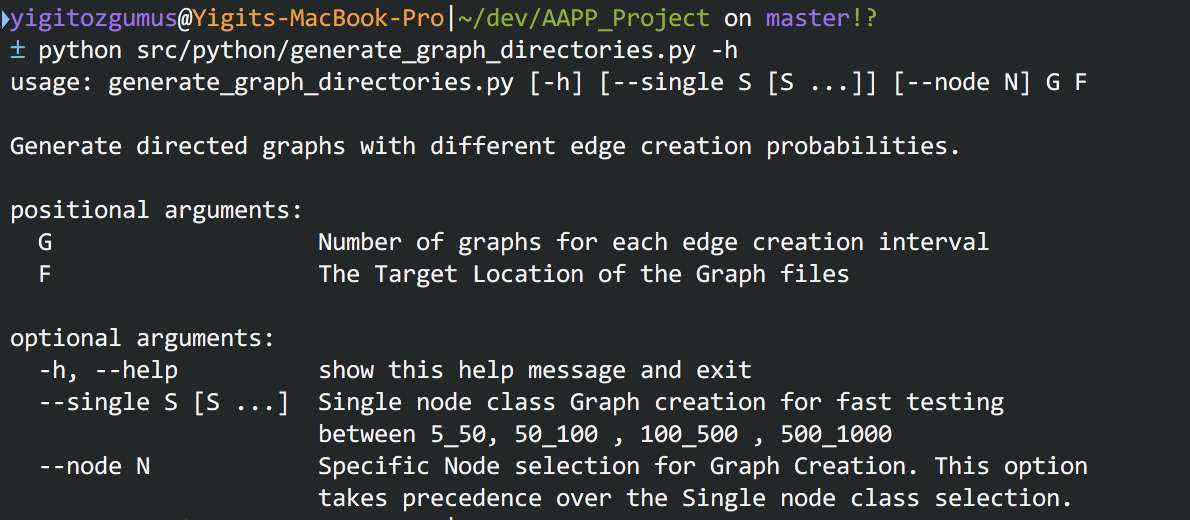
\includegraphics[width=1\textwidth]{generate}
				\caption{generate graph directories script help command result}
			\end{figure}
		\end{frame}
		\subsection{C++}
		\begin{frame}
			\frametitle{C++ Part}
			\begin{itemize}
				\item <1-6> Application Class uses:
				\begin{itemize}
					\item <2-6> Analyzer, Visualize and Session Classes
				\end{itemize}
				\item <3-6> Analyzer Class uses:
				\begin{itemize}
					\item <4-6> Nuutila, Pearce, Tarjan, Timer and GraphComponent Classes
				\end{itemize}
				\item <5-6> StorageItems struct is used by all algorithm classes to transfer the execution data 
			\end{itemize}
			\only<6>{	
			\begin{figure}[h!]
				\centering
				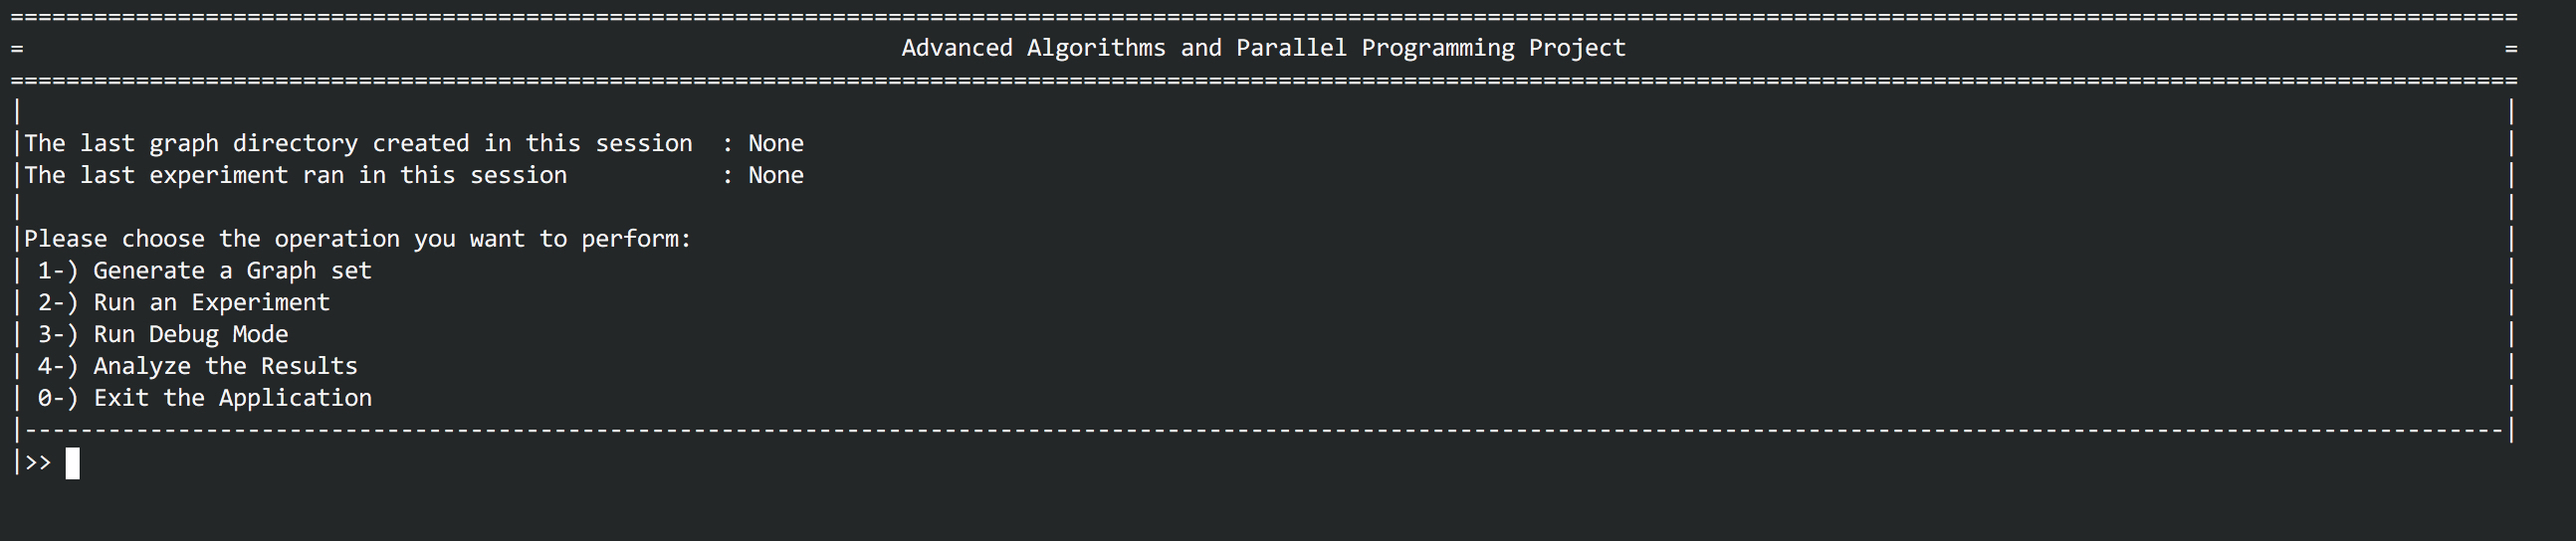
\includegraphics[width=1\textwidth]{application}
				\caption{The main screen of the Application}
			\end{figure}	
		}
		\end{frame}
	\section{Analysis of Results}
			\subsection{Results with respect to Storage Usage}
			\begin{frame}
				\frametitle{Analysis result of the first 5000 Graphs}
					\begin{figure}[h!]
					\centering
					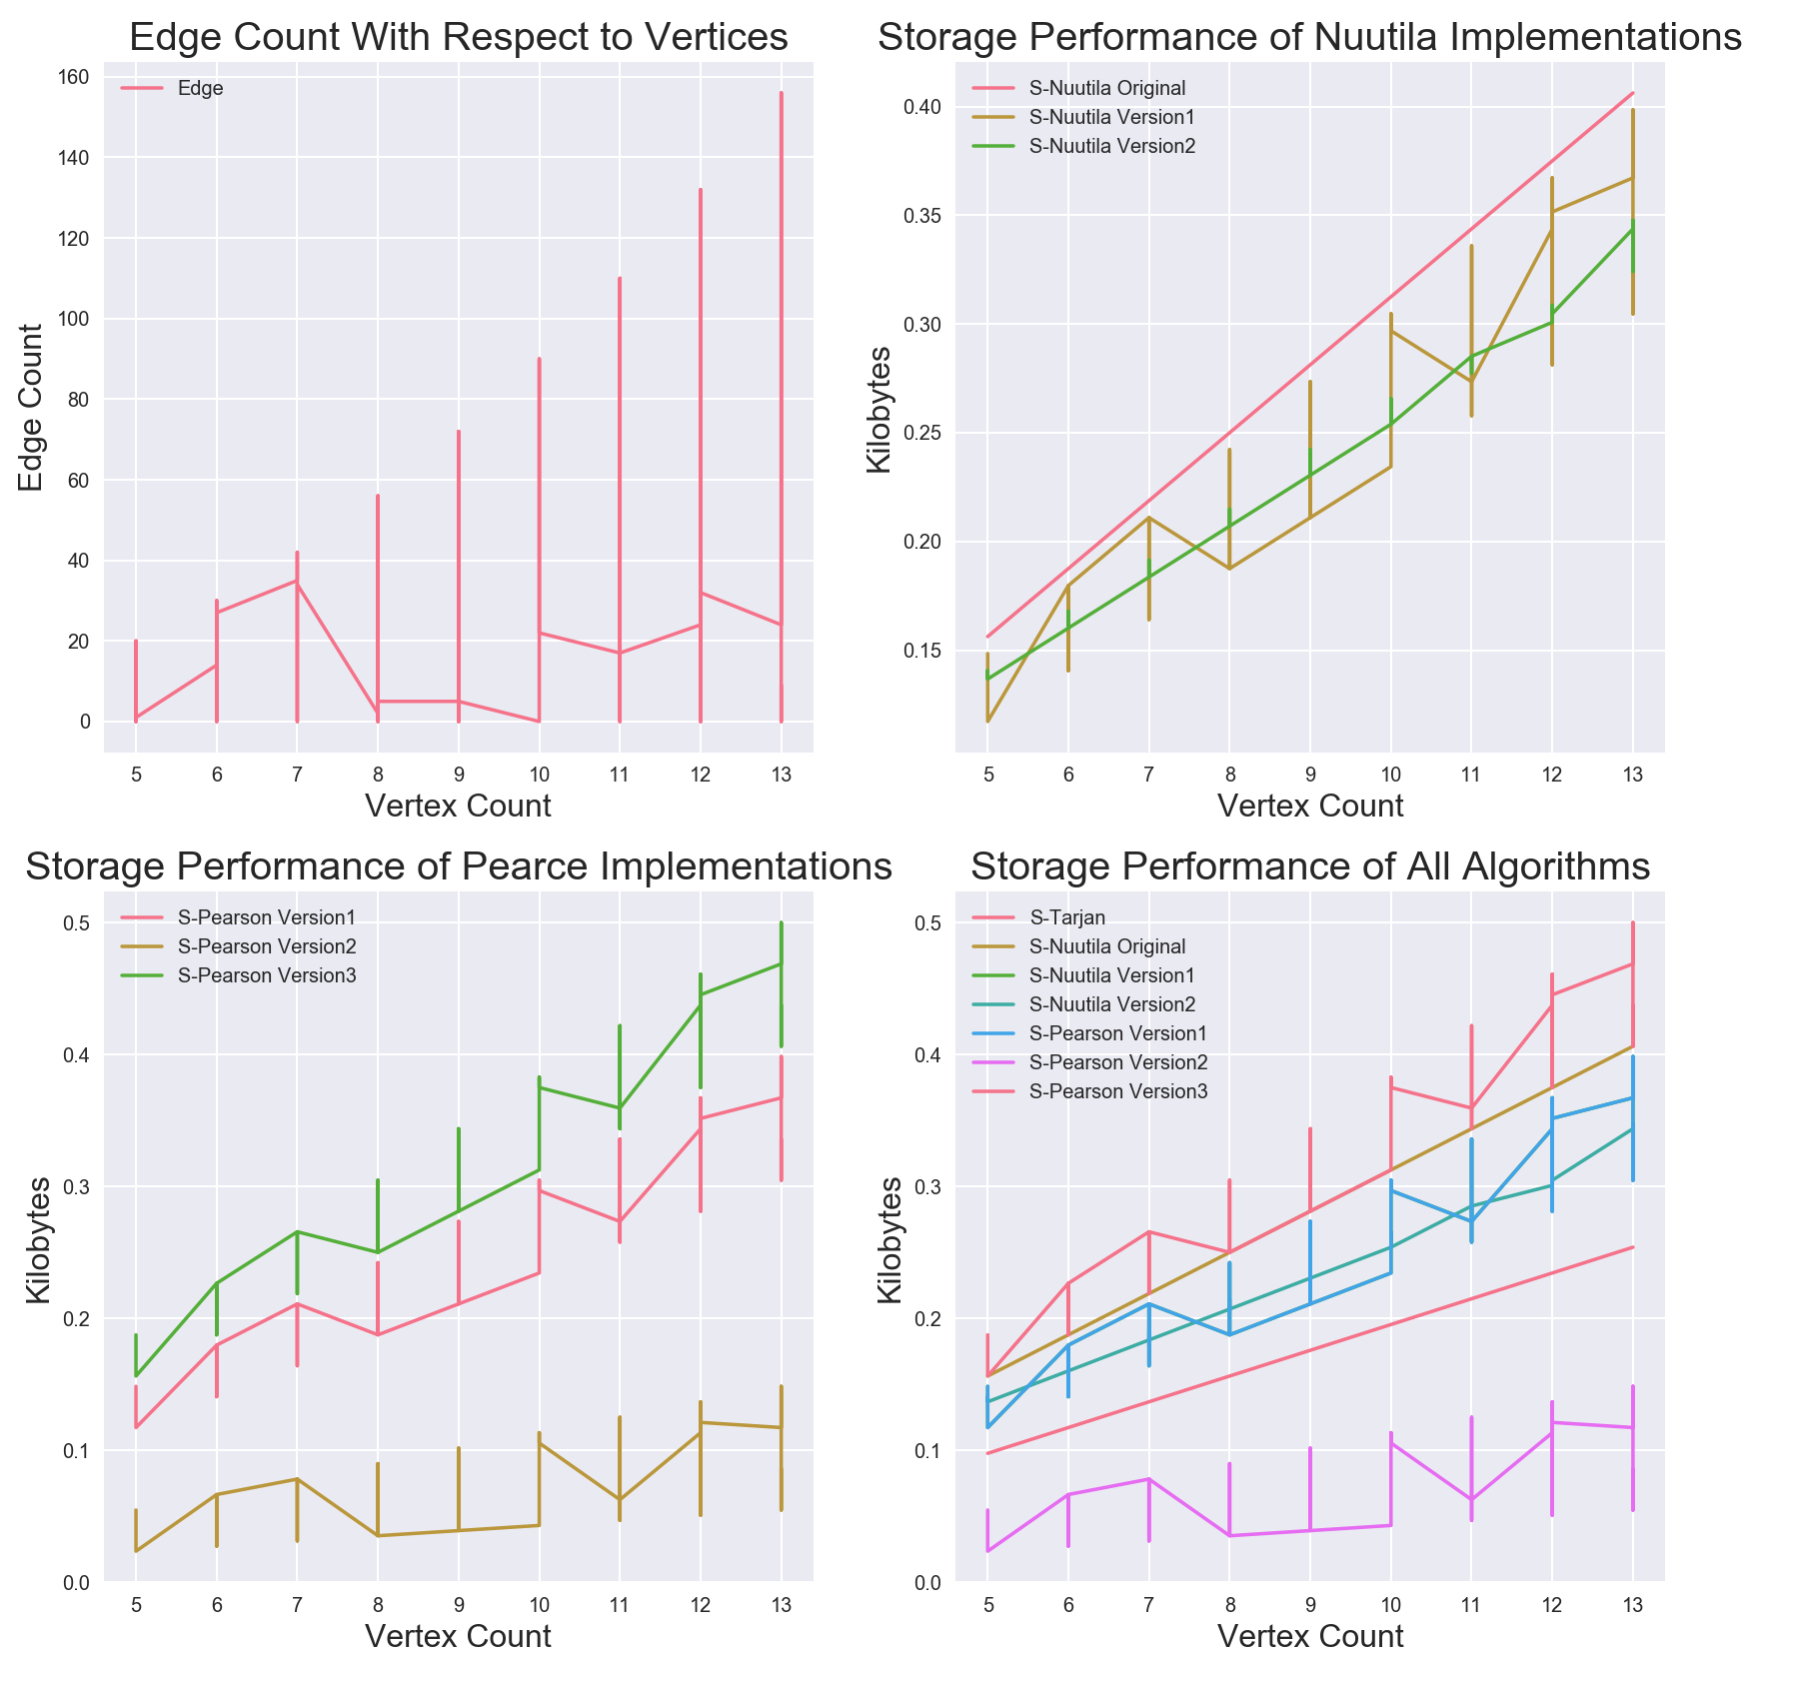
\includegraphics[width=0.7\textwidth]{S5000}
					\end{figure}
			\end{frame}
			
			\begin{frame}
				\frametitle{Analysis result of the first 10000 Graphs}
					\begin{figure}[h!]
					\centering
					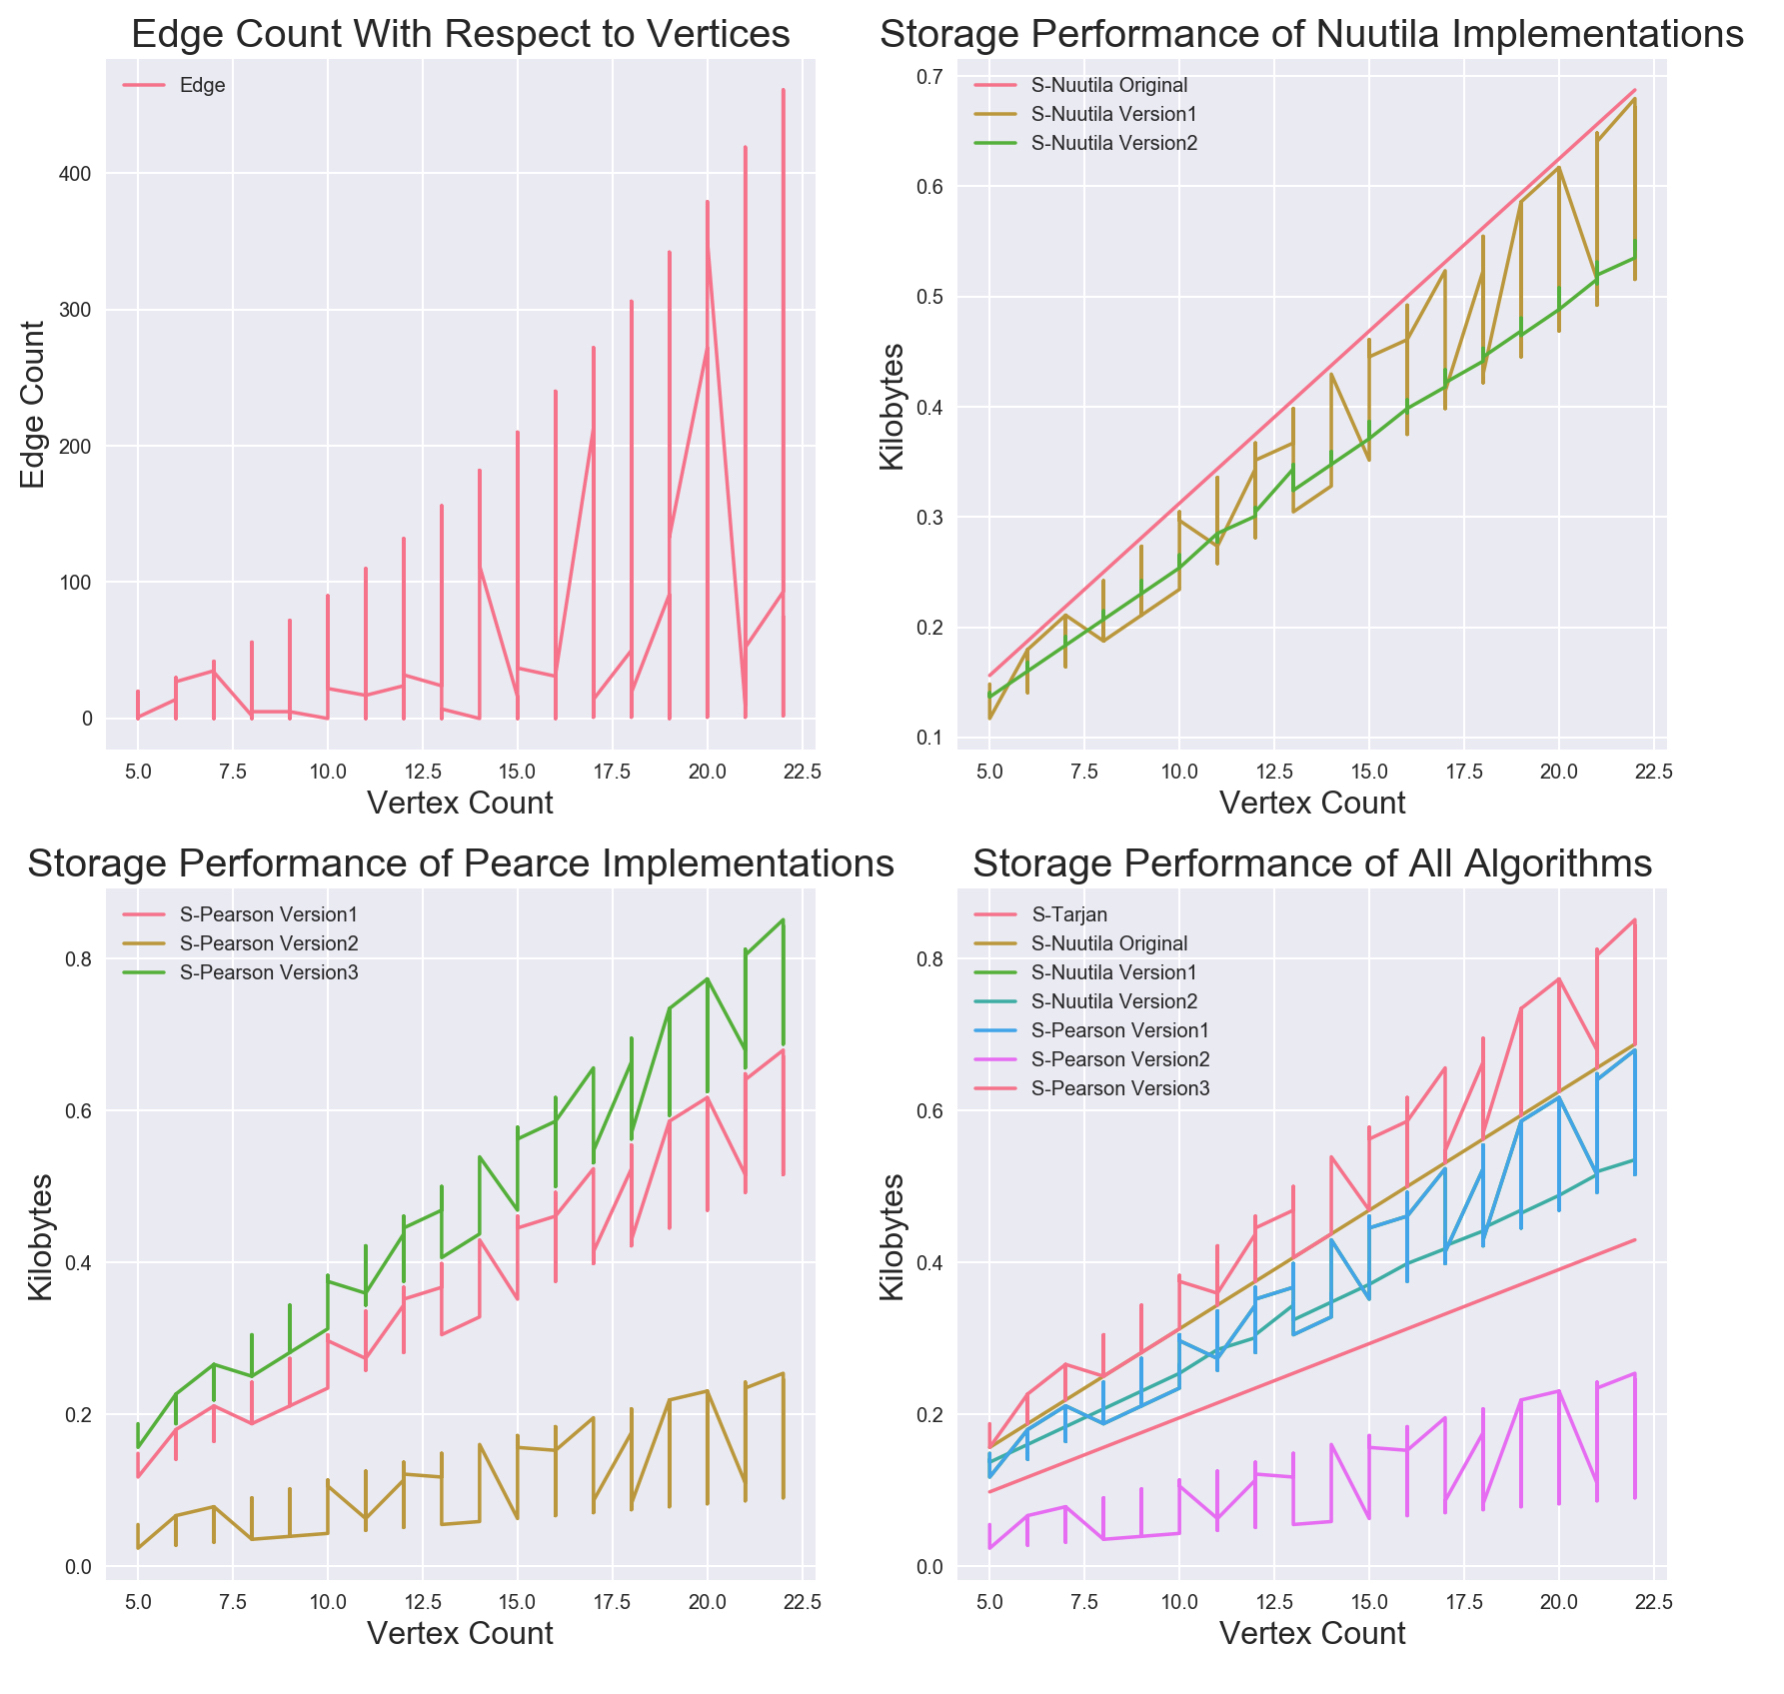
\includegraphics[width=0.7\textwidth]{S10000}
				\end{figure}
			\end{frame}
			\begin{frame}
				\frametitle{Analysis result of the first 15000 Graphs}
				\begin{figure}[h!]
					\centering
					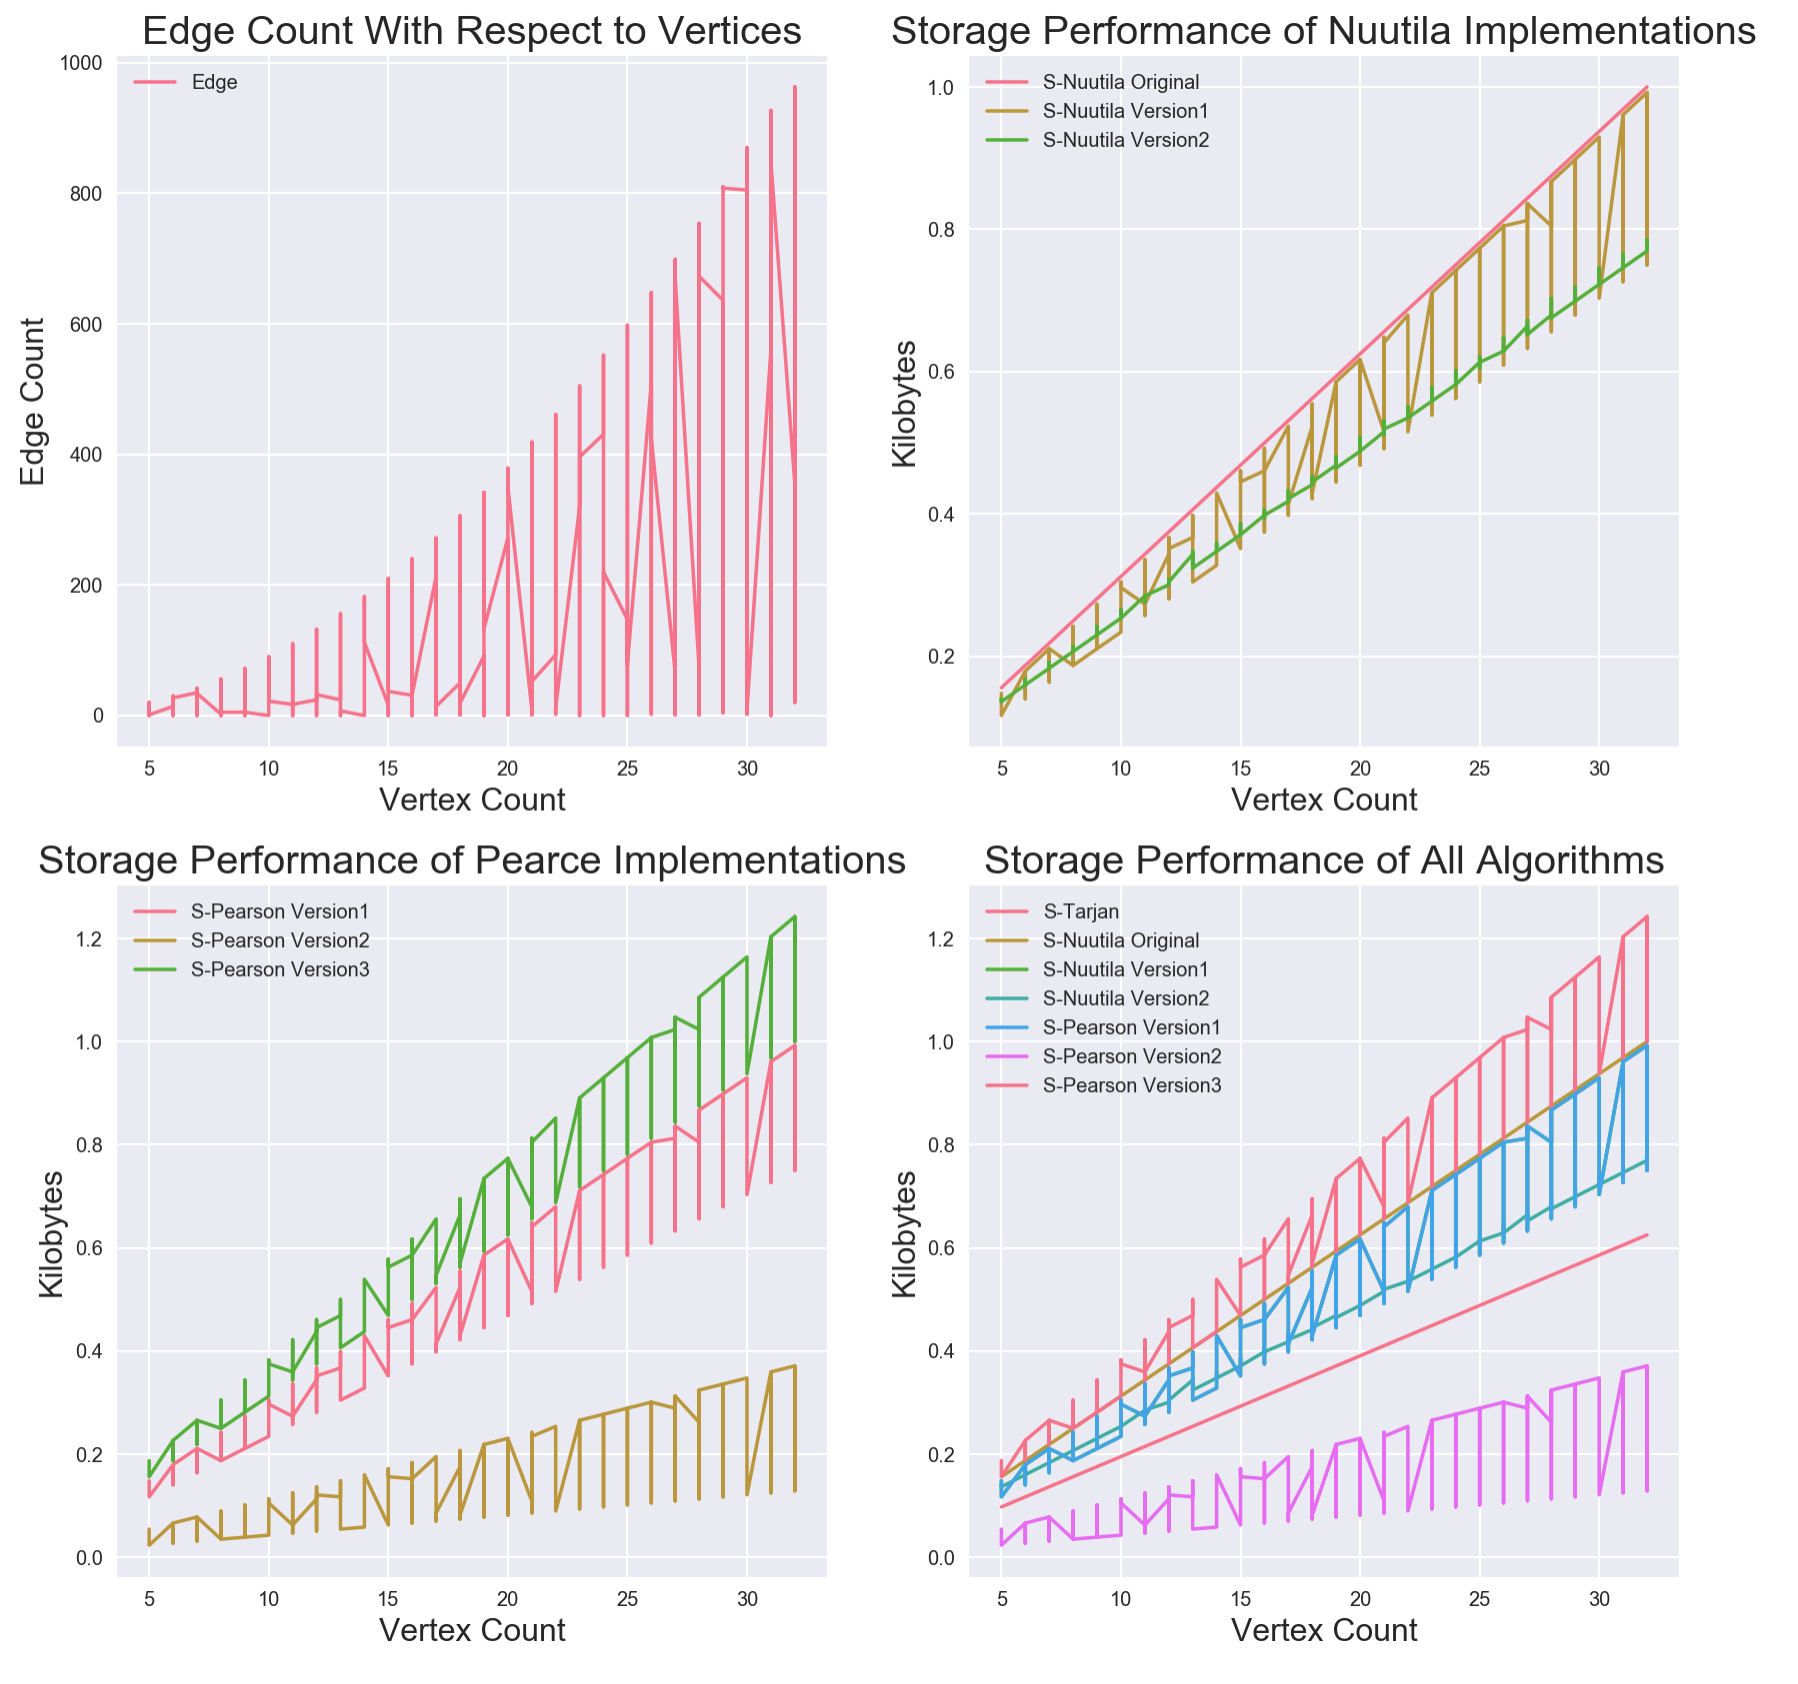
\includegraphics[width=0.7\textwidth]{S15000}	
				\end{figure}
			\end{frame}
			\begin{frame}
				\frametitle{Analysis result of the first 25000 Graphs}
				\begin{figure}[h!]
					\centering
					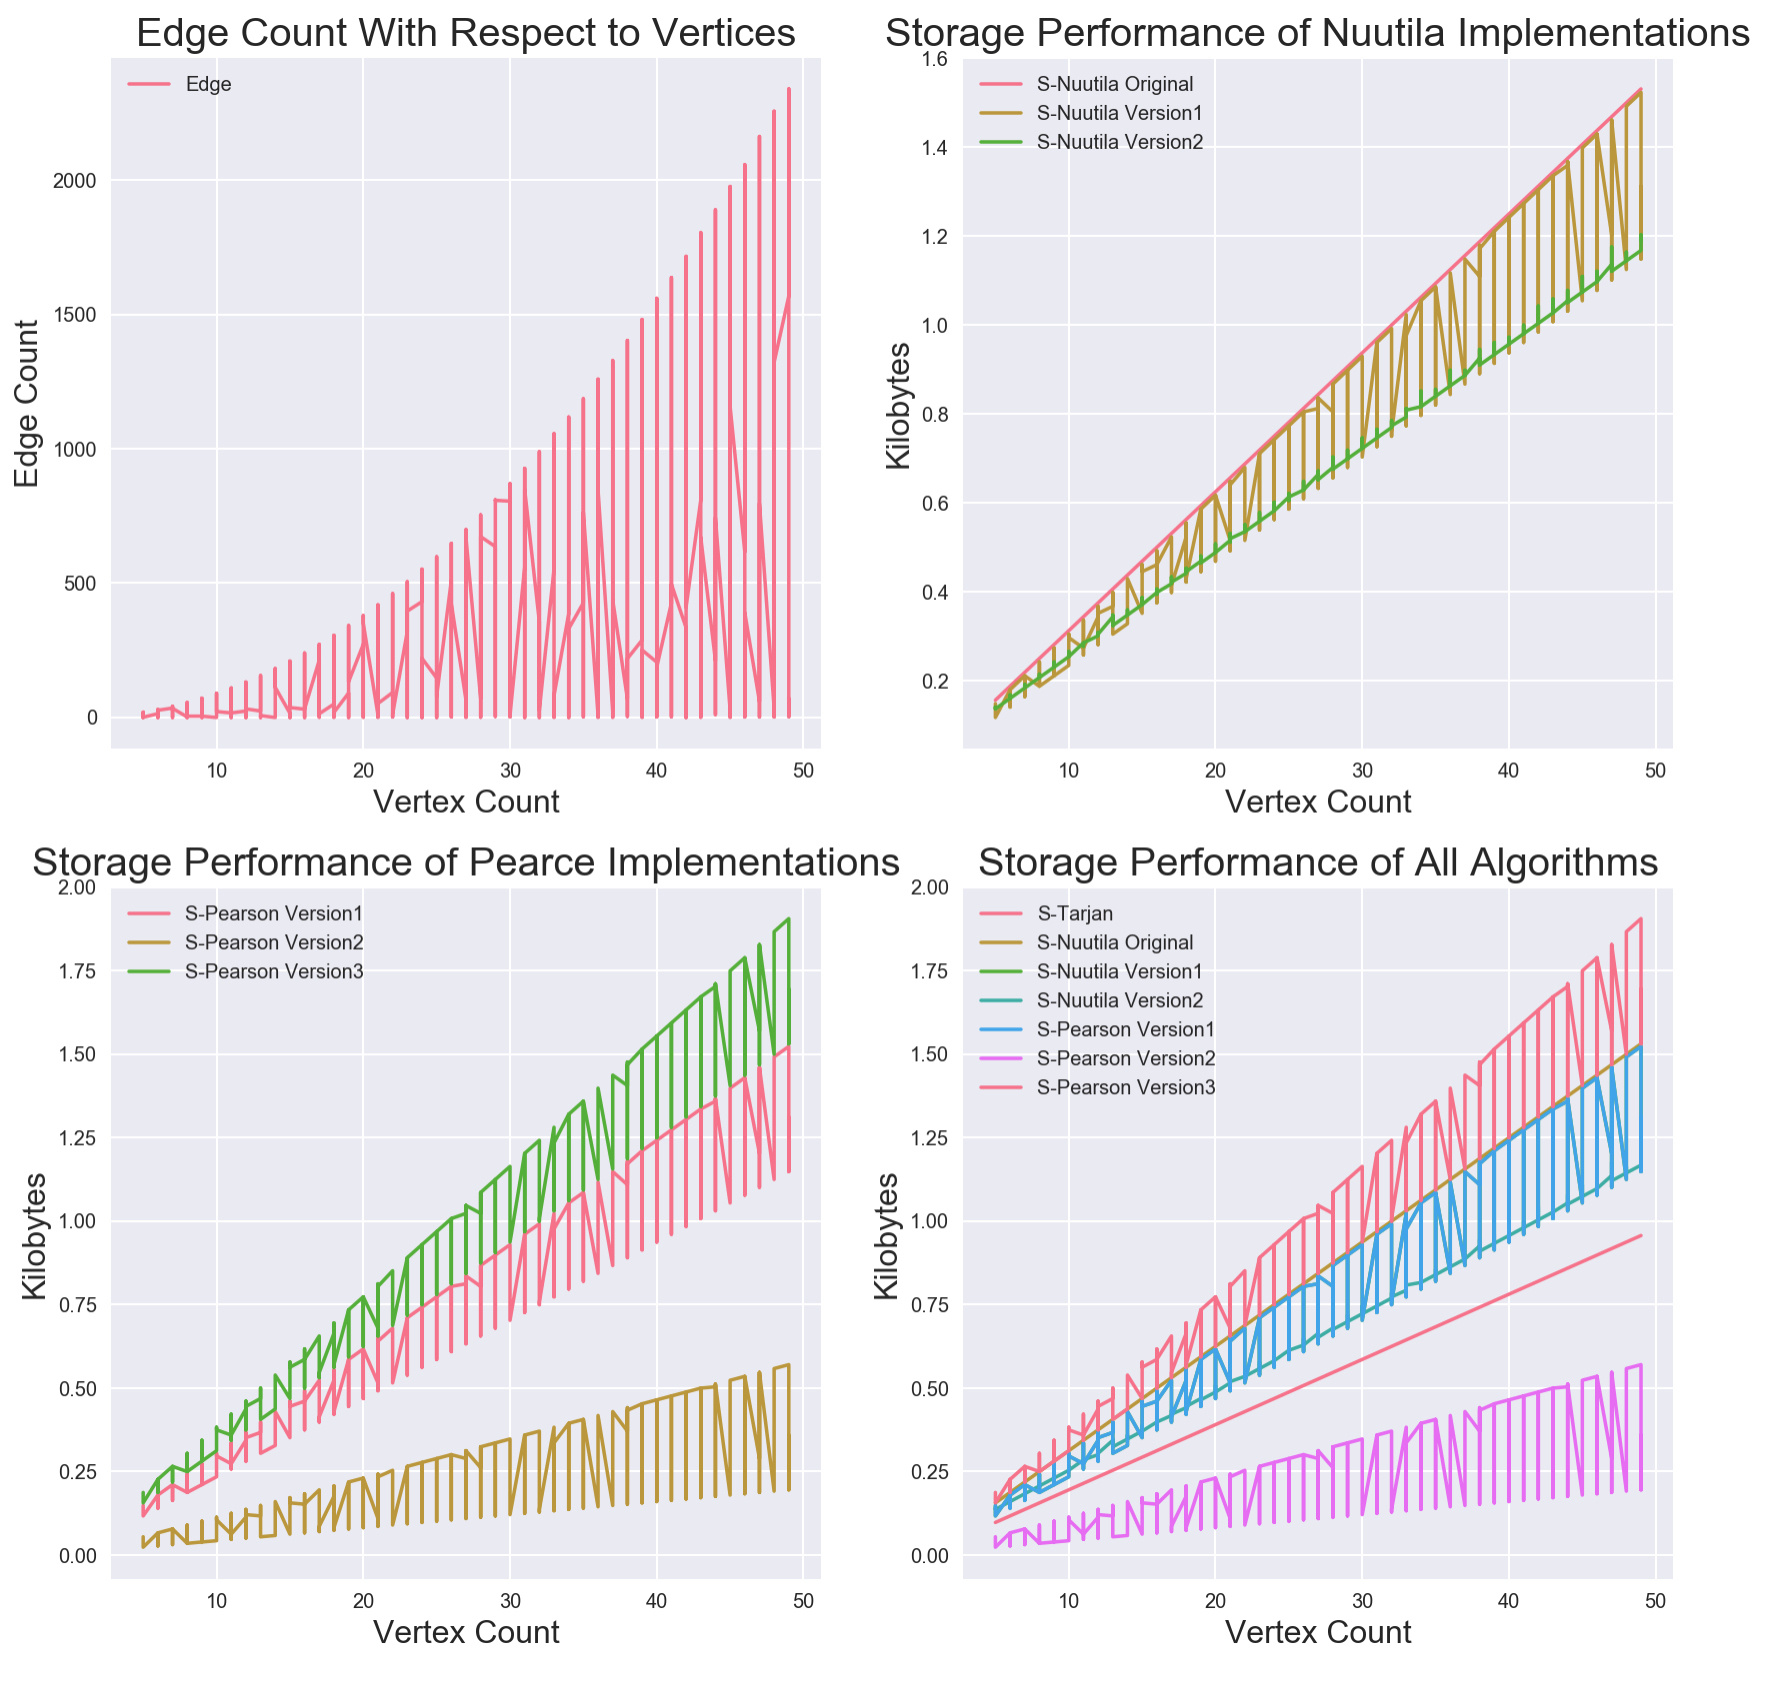
\includegraphics[width=0.7\textwidth]{S25000}
				\end{figure}
			\end{frame}
			\begin{frame}
				\frametitle{Analysis result of the first 50000 Graphs}
				\begin{figure}[h!]
					\centering
					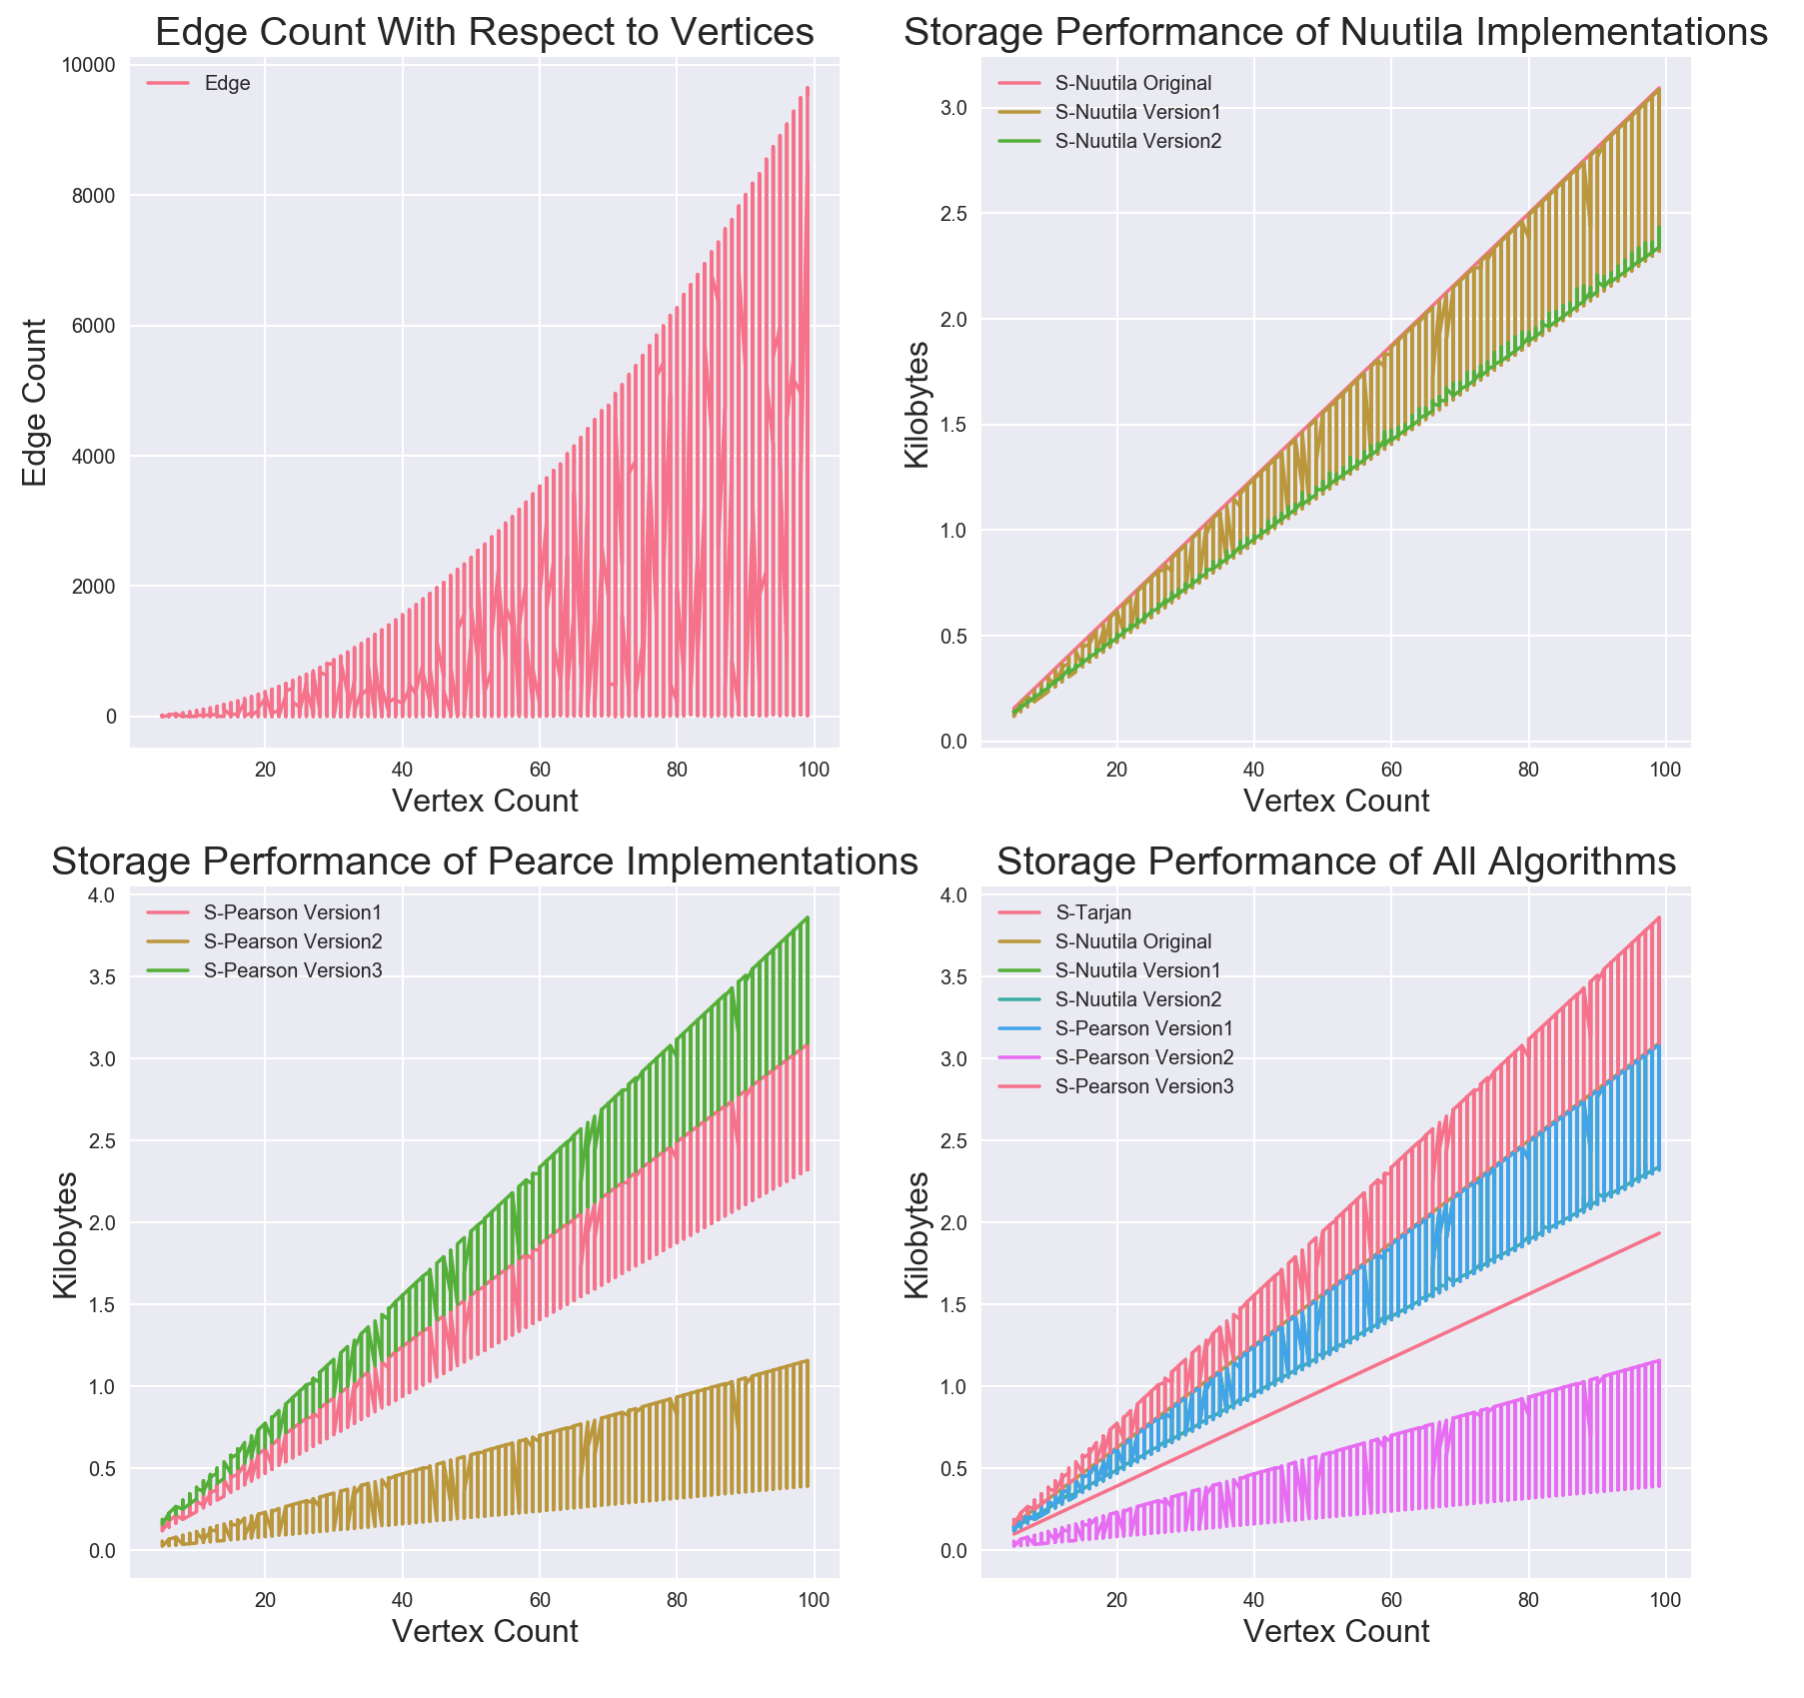
\includegraphics[width=0.7\textwidth]{S50000}
				\end{figure}
			\end{frame}
			\begin{frame}
				\frametitle{Analysis result of the first 75000 Graphs}
					\begin{figure}[h!]
					\centering
					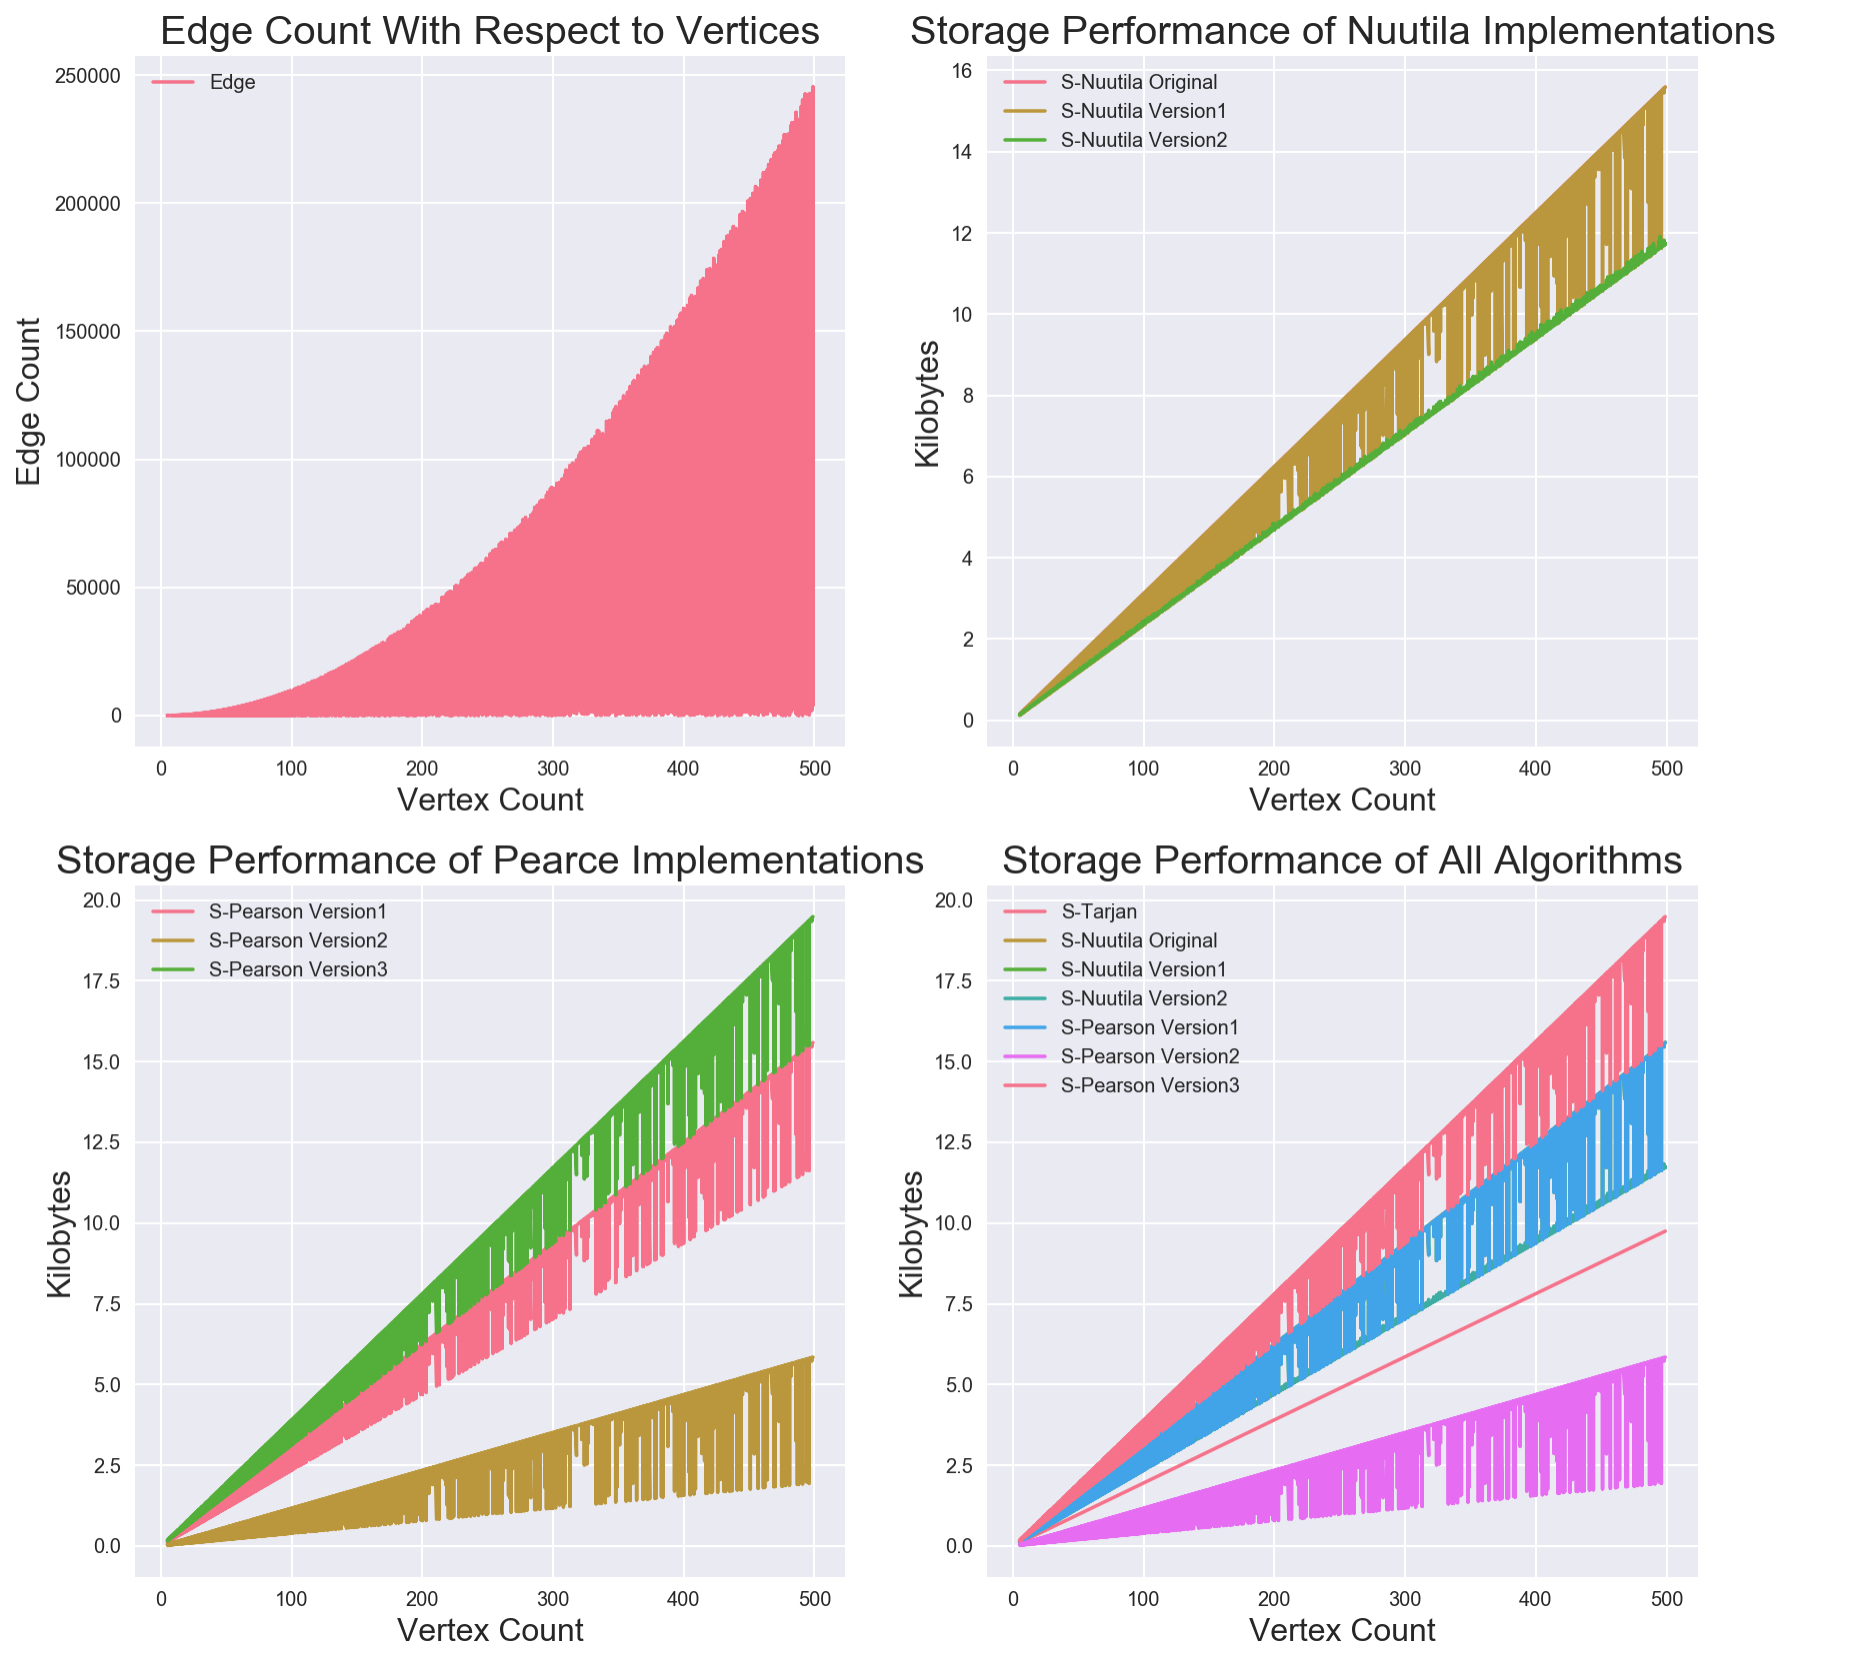
\includegraphics[width=0.7\textwidth]{S75000}
					\end{figure}
			\end{frame}
			\begin{frame}
				\frametitle{Analysis result of all of the Graphs}
				\begin{figure}[h!]
					\centering
					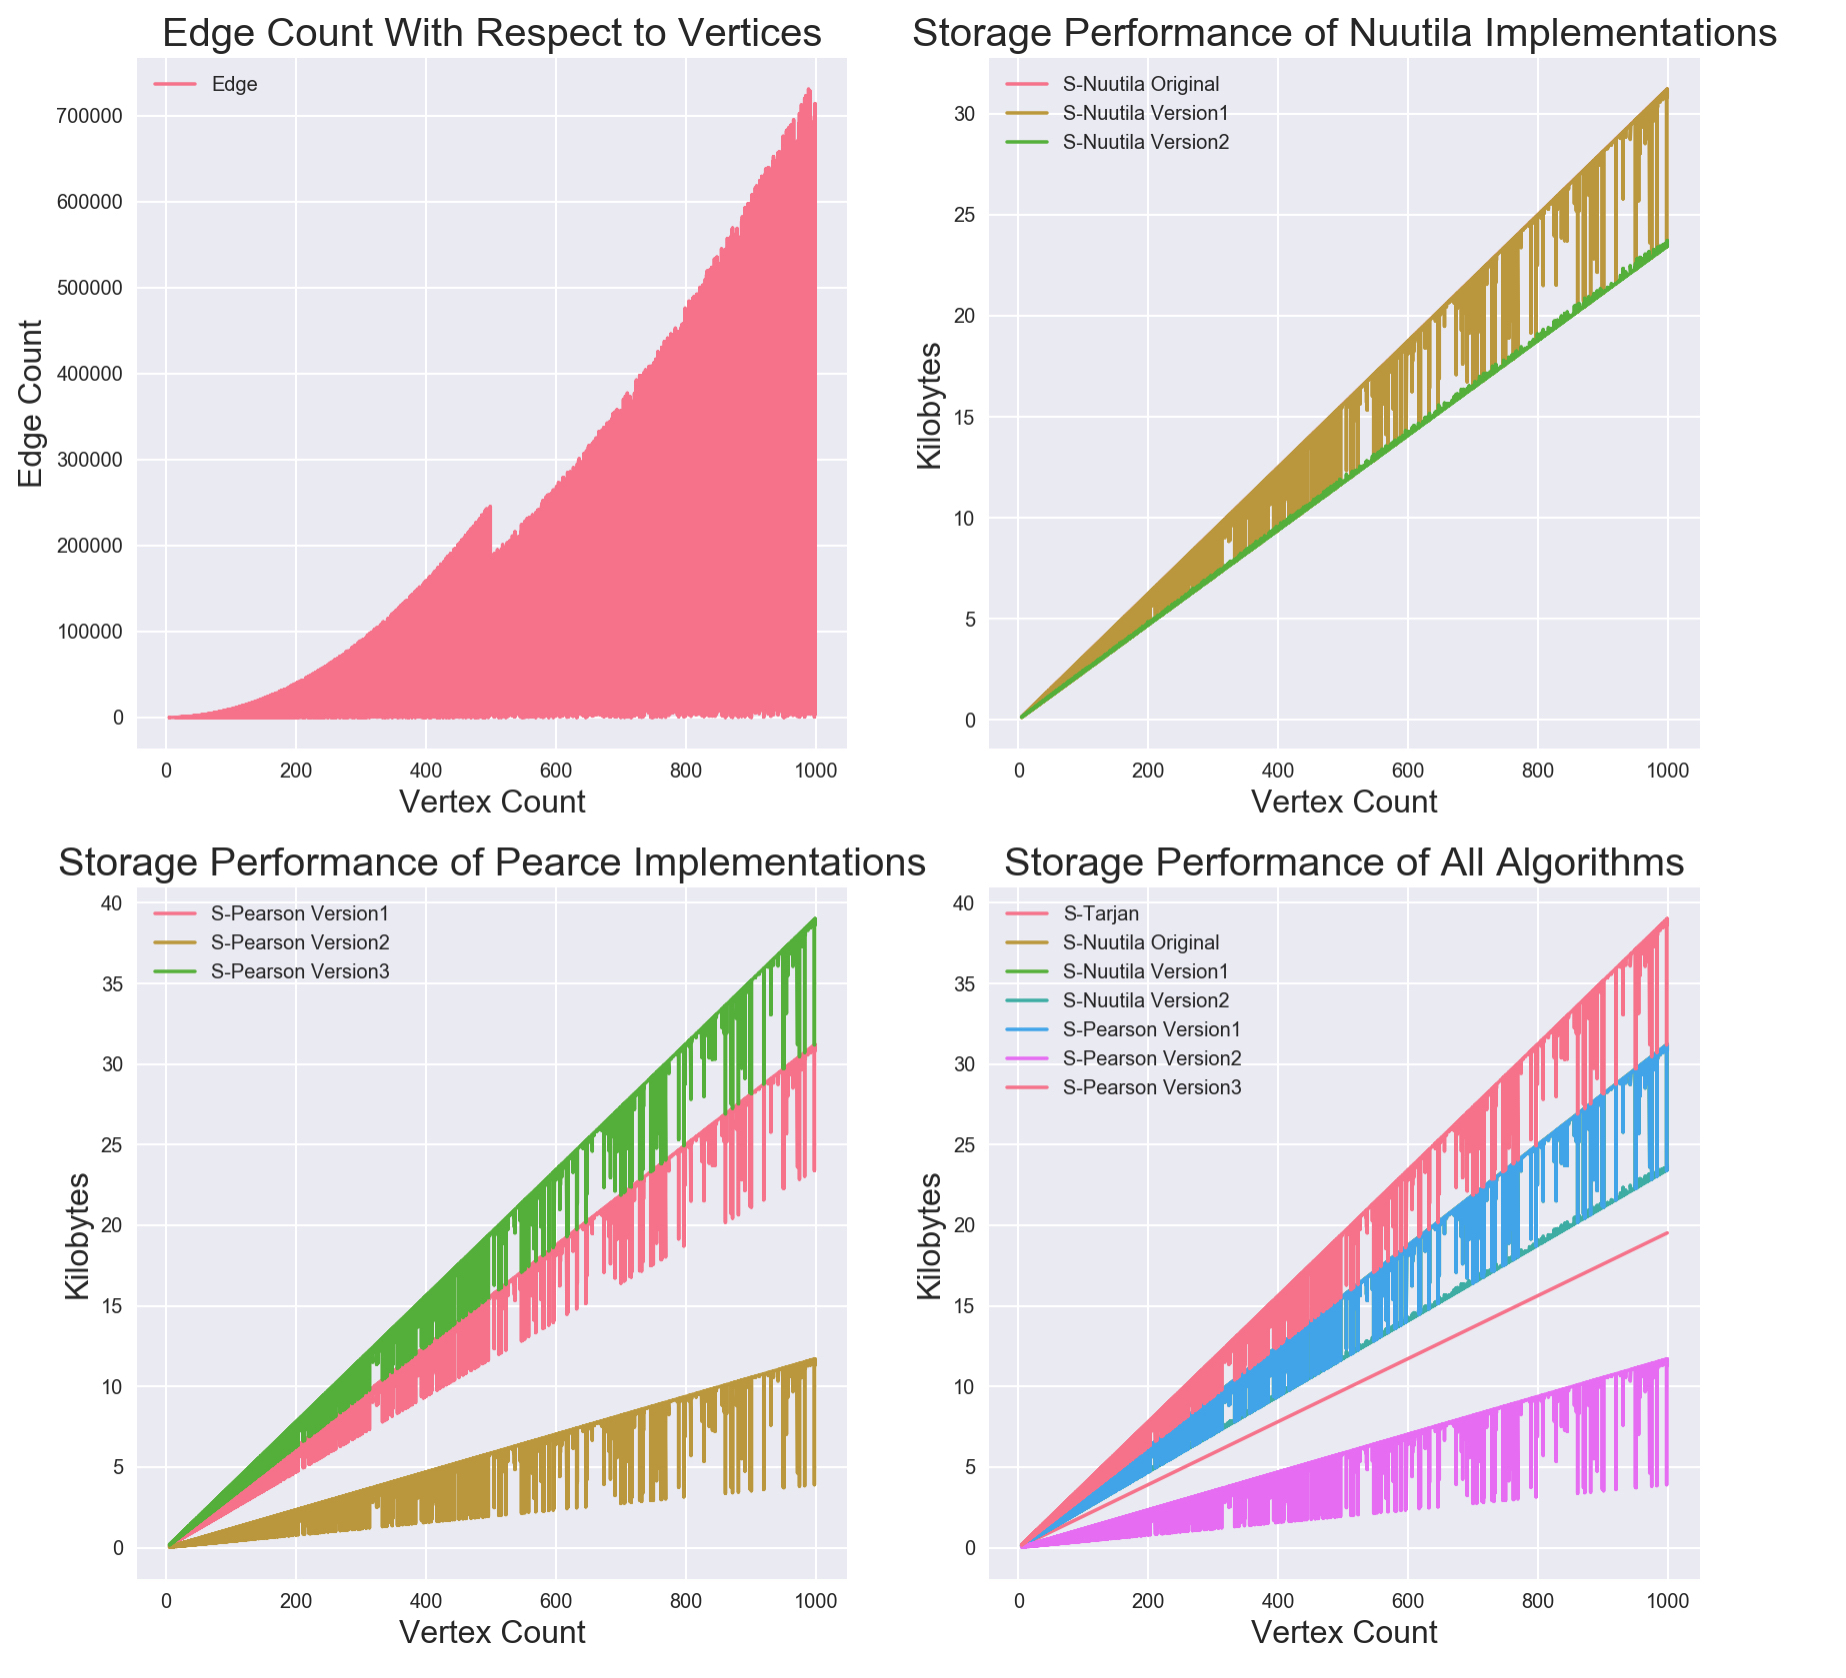
\includegraphics[width=0.7\textwidth]{SALL}
				\end{figure}
		\end{frame}
	\begin{frame}
		\frametitle{Analysis Results}
		\begin{itemize}
			\item <1-> For Nuutila algorithms, Version 2 uses the least amount of storage. 
			\item <2-> For Pearce algorithms, Version 2 Uses the least amount of storage.
			\item <3-> Among all the algorithms, Pearce Version 2 uses the least amount of storage .
		\end{itemize}
	\end{frame}
	\begin{frame}
		Demo ?
	\end{frame}
\end{document}